\chapter{Implementation}\label{chap4}
Authentication is a process of identification and verification of the user's access to the application. Authorization is a process of granting or denying access to the application based on the authorized user's identity and the permissions for that identity. \cite{auth-def} In this chapter, I will describe the implementation of those two processes for the client side along with the role-based access control described in the third chapter.\\
My implementation uses the authentication microservice that was designed and described along with the general authorization flow for this service by Ing. Andrii Plyskach in his master thesis \cite{mt-plyskach}. For the purpose of reducing security vulnerabilities, I will also describe a few adjustments to the functionalities of that microservice.

%%%%%%%%%%%%%%%%%%%%%%%%%%%%%%%%%%%%%%%%%%%%%%%%%%%%%%%%%%%%%%%%

\section{Used software} The technologies used for the development of the BI-DBS portal are described in section 1.3. In this section I will mention which of them I have used for the implementation part of this thesis and also describe the used libraries.\\
The UI is implemented in Vue.js \cite{vue-docs} together with the Quasar framework \cite{quasar-doc} for creating good-looking components and Typescript \cite{typescript-doc} as a programming language. 

\subsection{Pinia.} Pinia is a reactive state management library. It allows to easily update data and react to changes in the application's state. Besides, it provides type safety and thus integrates well with Typescript. In my implementation I have used it for storing the state of users' authorization along with the user's identity information such as their role. \cite{pinia-docs}

\subsection{Router} Vue Router is a routing library that provides mapping URLs to the components, allowing SPA to load pages based on the given URL dynamically. I have used it for managing access to the components based on the user's authentication state and identity. More about role-based access control is in section 4.3. \cite{router-doc}

\subsection{Axios} Axios is a Javascript library for making HTTP requests from the browser of various request methods. It automatically transforms the response data to its response type and allows it to intercept requests and responses. I have used it for communication with the backend. \cite{axios-docs}



%%%%%%%%%%%%%%%%%%%%%%%%%%%%%%%%%%%%%%%%%%%%%%%%%%%%%%%%%%%%%%%%

\section{Authentication and authorization}
Authentication and authorization processes are implemented using the secure OAuth 2.0 protocol \cite{oauth}. The whole procedure is based on communication and data exchange between four roles and components: the resource owner(user) the client app, the authorization server and the authorization microservice.

\subsection{OAuth protocol}
OAuth protocol is a modern industry-standard protocol for authorization. 
In general, the OAuth protocol enables users to provide a client with secure access to server resources and without a need for users to share their credentials directly with an application they want to access. OAuth is widely used by major companies to allow users to grant access to their resources to trusted third-party applications. \cite{oauth} This protocol is also obviously suitable for university applications and the BI-DBS portal in particular.

\subsection{Tokens} Token in this context is a string that has some value for authentication and authorization processes. In the implementation, the client gets the authorization code from the authorization server and exchanges it for access and refresh tokens with the server. 

\subsubsection{Access token}
The OAuth protocol uses an access token to represent the authorization status in the application. The access token is a short-time living token used to verify the user's access to the application. \cite{access-token} An access token is sent in every HTTP request made to the server. Thus the server can verify if the token is valid and then complete a request. It can be used for communication with the application server until that token expires. The expiration time is set to one hour. \\ 
The implementation uses a JWT token type for creating the access token. 
 
\paragraph*{JWT token.} JSON web token(JWT) is a token type standard that allows securely transmitting JSON objects. It consists of three parts: header which specifies the algorithm used to sign the token, payload containing the data being sent and signature that validates the token's integrity and assures it has not been modified. \cite{jwt-token}

\begin{figure}[hp]
\centering
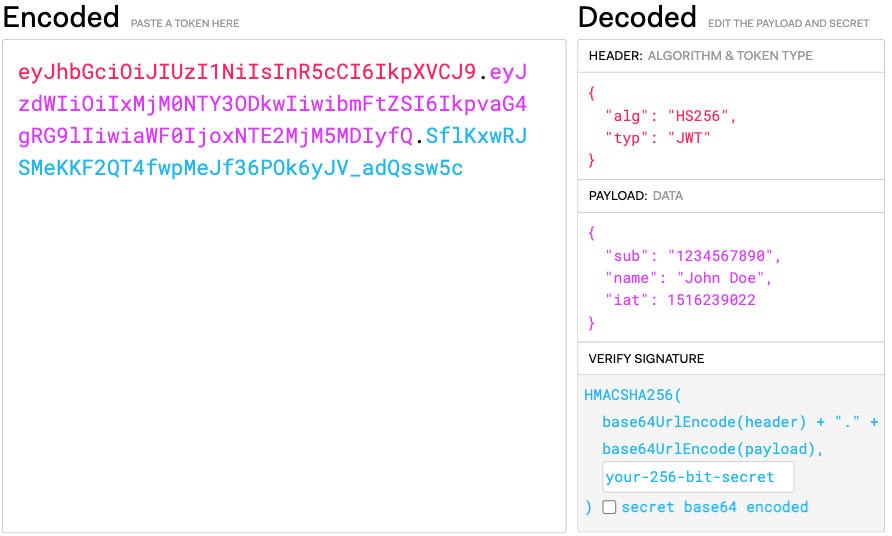
\includegraphics[scale=0.38]{../png/jwt_token.png}
\caption{Example of encoded and decoded JWT token from jwt.io. \cite{jwt-token}}
\label{jwt}
\end{figure}



\subsubsection{Refresh token} Refresh token is a type of token used for requesting a new access token when the current one expires. It is a long-time living token because it is meant to live longer than an access token due to its existence purpose. With the help of a refresh token user does not need repeatedly log in every hour which helps to improve user experience. \cite{refresh-token}


\subsection{Authorization server} The authorization server is a key component of the authorization and authentication processes based on the OAuth 2.0 protocol. 
For the authentication and authorization in the BI-DBS portal, we use the faculty's authorization server called Zuul OAAS. It is open-source and available for anybody from CTU. \cite{auth-server} Zuul OAAS provides three endpoints:

\begin{itemize}
    \item \emph{Authorization endpoint: /oauth/authorize.} It is used for the authentication and authorization processes of a user. It displays the login form for a user and after the submission of that form, it validates credentials and in a case of success does a redirect back to the BI-DBS client app server with the authorization code. 
    \item \emph{Token Endpoint: /oauth/token.} This endpoint provides us with two important functionalities:
        \begin{itemize}
            \item Exchanging authorization code from the authorization endpoint for access and refresh tokens.
            \item Generating new access token by accepting the refresh token.
        \end{itemize}
   \item \emph{Check Token Endpoint: /oauth/check\_token.} For controlling the validity of the token, the authorization server provides this endpoint which checks the token for being valid.
\end{itemize}

\noindent With the use of these endpoints we have constructed the authentication and authorization processes, which are more deeply described in \ref{sec425} and shown in Figure \ref{access}.


\subsection{Apps manager} To communicate with the authorization server, the application must be registered in the Apps Manager \cite{app-manager}. For further communication with the server we will need three parameters: client id, client secret and redirect URL. The first two parameters are generated by the app manager. These are simplified login and password for our application. But the redirect URL can be set to the URL we want, this URL will be used for the redirect back to our application after the successful authorization of a user. These parameters are used as a part of the HTTP requests, that frontend and backend send to the authorization server. 

\begin{figure}[hp]
\centering
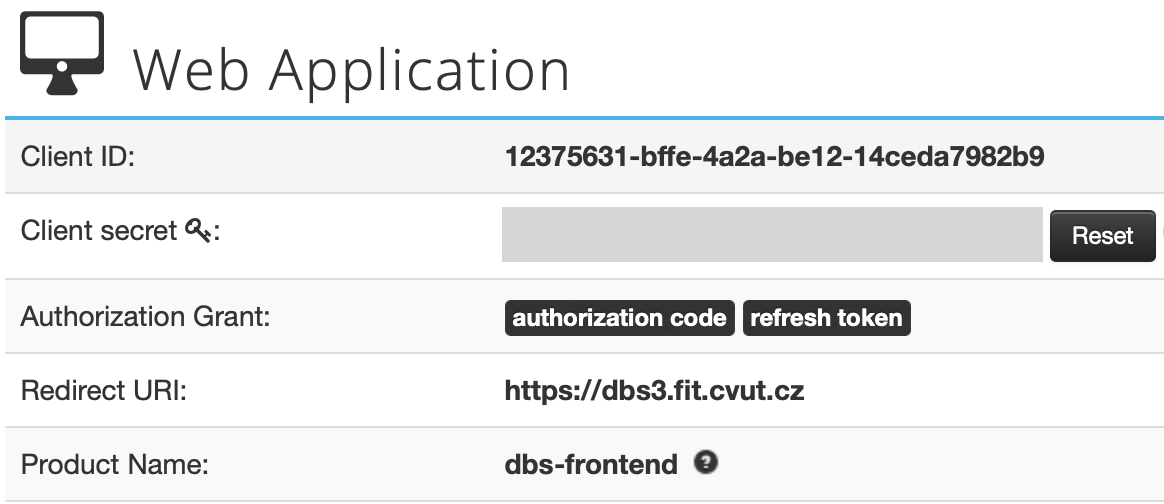
\includegraphics[scale=0.52]{../png/app_manager.png}
\caption{The example of the application registry in the App Manager \cite{app-manager}}
\label{appm}
\end{figure}


\subsection{Authentication and authorization flow}\label{sec425} For better visualization I have provided the implicit flow of the implemented services and a sequential diagram in Figure \ref{access}.\\

\noindent \textbf{Explicit flow:}

\begin{enumerate}
    \item Unauthorized user is trying to access the application and access validation redirects a user to the login page.
    \item By clicking on the login button user gets transferred to the page provided by the authorization server with a form for submitting credentials.
    \item After submitting credentials authorization server redirects the user back to the BI-DBS client with an authorization code which the client exchanges with the backend for the JWT access and refresh tokens.
    \item Finally the user is redirected to the page they wanted to access.
\end{enumerate}

\begin{figure}[hp]
\centering
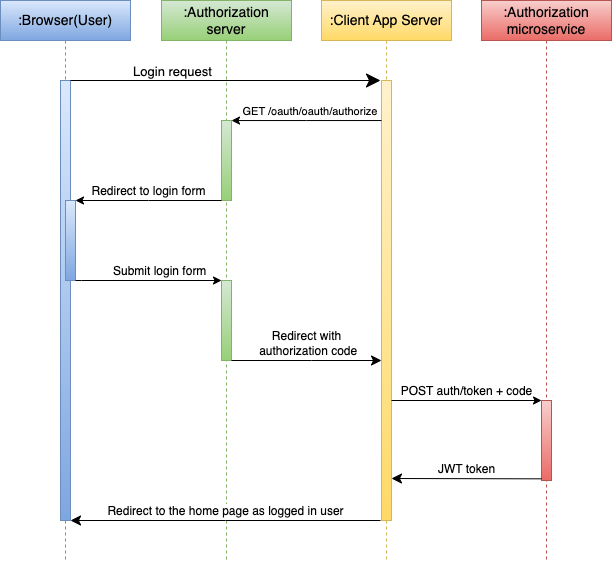
\includegraphics[scale=0.56]{../png/generate_token.png}
\caption{Sequential diagram of generating an access token}
\label{access}
\end{figure}



\subsection{Refresh token flow} Another very important part of the implementation is refreshing the access token with the usage of the refresh token. A user does not know about that process and does not participate in it. This process replaces the constant logging in by a user, which improves security since a user does not need to enter credentials repeatedly and also does not annoy or interrupt a user. The explicit flow and sequential diagram of the token refreshing process in Figure \ref{refresh} are provided for showing the implementation details.\\

\noindent \textbf{Explicit flow:}

\begin{enumerate}
    \item A user who has already been authorized in the application is trying to make a request. However, the access token has expired and cannot be used anymore for the requests.
    \item The client detects that the access token has expired and sends a request to the authorization microservice for a new access token in exchange for the current access token and the refresh token.
    \item After receiving a new access token client completes the request for a user with the usage of that access token.
\end{enumerate}

\begin{figure}[hp]
\centering
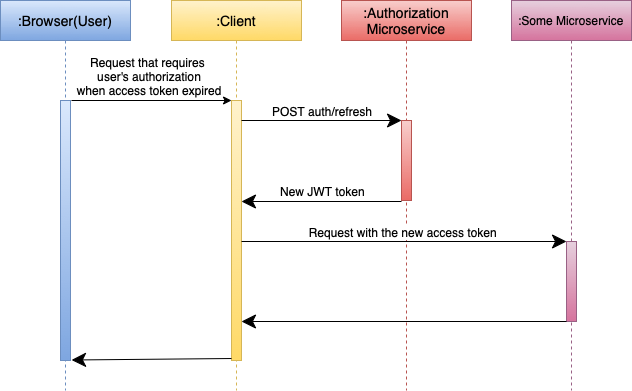
\includegraphics[scale=0.6]{../png/refresh_token.png}
\caption{Sequential diagram of refresh an access token using refresh token}
\label{refresh}
\end{figure}


%%%%%%%%%%%%%%%%%%%%%%%%%%%%%%%%%%%%%%%%%%%%%%%%%%%%%%%%%%%%%%%%

\section{Security} Needles to say that the development process comes together with analyzing security vulnerabilities and implementing the solution to reduce them. My implementation contains two points where the setup plays a big role: the solution for storing sensitive data such as access and refresh tokens and the configuration of communication between the client and server sides.


\subsection{Tokens storage} Access and refresh tokens are both very sensitive pieces of data. In the case of successfully stealing the refresh token, an attacker will get long-term access to the application, or a short term in the case with the access token. That is why it is important to store these tokens as securely as it is possible.\\

\noindent \textbf{Most common attacks:} 

\begin{itemize}
    \item \emph{Cross-site scripting (XSS) attacks.} This is a type of attack where an attacker injects malicious scripts into a web page viewed by other users. It basically happens when an application trusts a user and the content, which can be inserted by them. 
    \item \emph{Cross-site request forgery (CSRF) attacks.} In general, this attack can be described as tricking a user into unintentionally performing some action. In this way, attackers just use the user's account to perform some harmful requests.
\end{itemize}


\noindent \textbf{Types of browser storages:} 

\begin{itemize}
    \item \emph{Local storage.} Local storage is web storage that allows the saving of key-value pairs of data. It provides the stored data persistence across the page reloading and can fit up to 5MB of data. Content from the local storage cannot be automatically sent and it makes it prone to CSRF attacks. However, it is not considered secure storage for keeping sensitive data due to the vulnerability to XSS attacks.
    \item \emph{Session storage} Session storage is client-base storage available by the browser which is very similar to the local storage. It has the same memory limit and vulnerabilities. But in addition to that it does not provide the persistence of data, which is a disadvantage to the user experience due to the need for repeated authentication.
    \item \emph{Cookies} Cookies are another way of storing data using a browser. Cookies can store much less data - up to 4KB, which might not always be enough for storing big tokens, but it is absolutely enough for my implementation. Cookies are vulnerable to both CSRF and XSS attacks, but with a proper configuration of secure attributes they are less vulnerable than local or session storage. Cookies can also be configured to be automatically sent with every HTTP request or some certain request.
\end{itemize}

\paragraph*{Solution for the refresh token.} The perfect solution for storing sensitive data in a browser does not exist and in order to keep the data secure there should be also implemented other vulnerability-reducing features like input data validation, escaping and others. However, with the proper use of security attributes, cookies are much more likely to mitigate those attacks. Moreover, using cookies for storing tokens is recommended by the OWASP community due to their secure configuration options. \\
I have come to the solution of storing the refresh token, which is the most sensitive token requiring persistence across page reloads, in httpOnly cookies. HttpOnly cookies must be set on the server side as they are not accessible for JavaSccirpt. Therefore, I had to adjust the implementation of sending and receiving the refresh token in the authentication microservice from the body of requests to cookies. Figure 4.5 shows the configuration of security attributes for the refresh token cookie.\\

\begin{figure}[h]
\centering
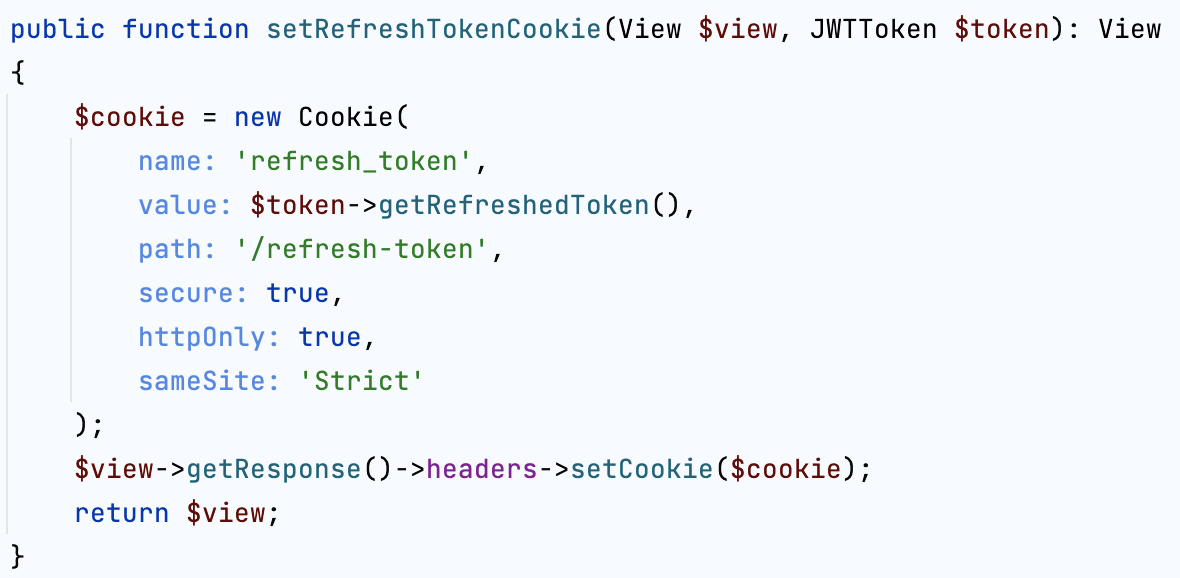
\includegraphics[scale=0.6]{../png/cookies.png}
\caption{Cookies setting}
\end{figure}

\noindent \textbf{Security attributes:}

\begin{itemize}
    \item \emph{Path.} URL path to which the cookie will be automatically sent.
    \item \emph{Secure.} This flag specifies that the cookie can be sent only through HTTPS ecrypted connections.
    \item \emph{HttpOnly.} The httpOnly flag is created to mitigate XSS attacks. With this flag, cookies can not be accessed by the Javascript.
    \item \emph{SameSite.} The strict value of that parameter means that the cookie is only sent if you are on the site that the cookie is set for. SameSite attribute is introduced for protection against CSRF. 
\end{itemize}


% https://www.invicti.com/learn/cookie-security-flags/

\paragraph*{Solution for the access token.} The access token is represented as JWT token, it contains the important information about the expiration time of the token and user's identity. It cannot be stored in the same way as refresh token as a client needs to have an access to that token directly.\\
Another way of storing the sensetive data which is considered more secure then local and session storages and cookies is storing it in memory(in a variable). This ways is considered more secure, because it is more prone to XSS attacks. The disadvantage of that method is that it doesn't provide the persistence, but in a case with access token it is a resolvable challenge.\\
First of all I have decided to store the access token and parsed information about user in the Pinia store, which is more secure then global variables. This store is shown in Figure 4.6.


\begin{figure}[h]
\centering
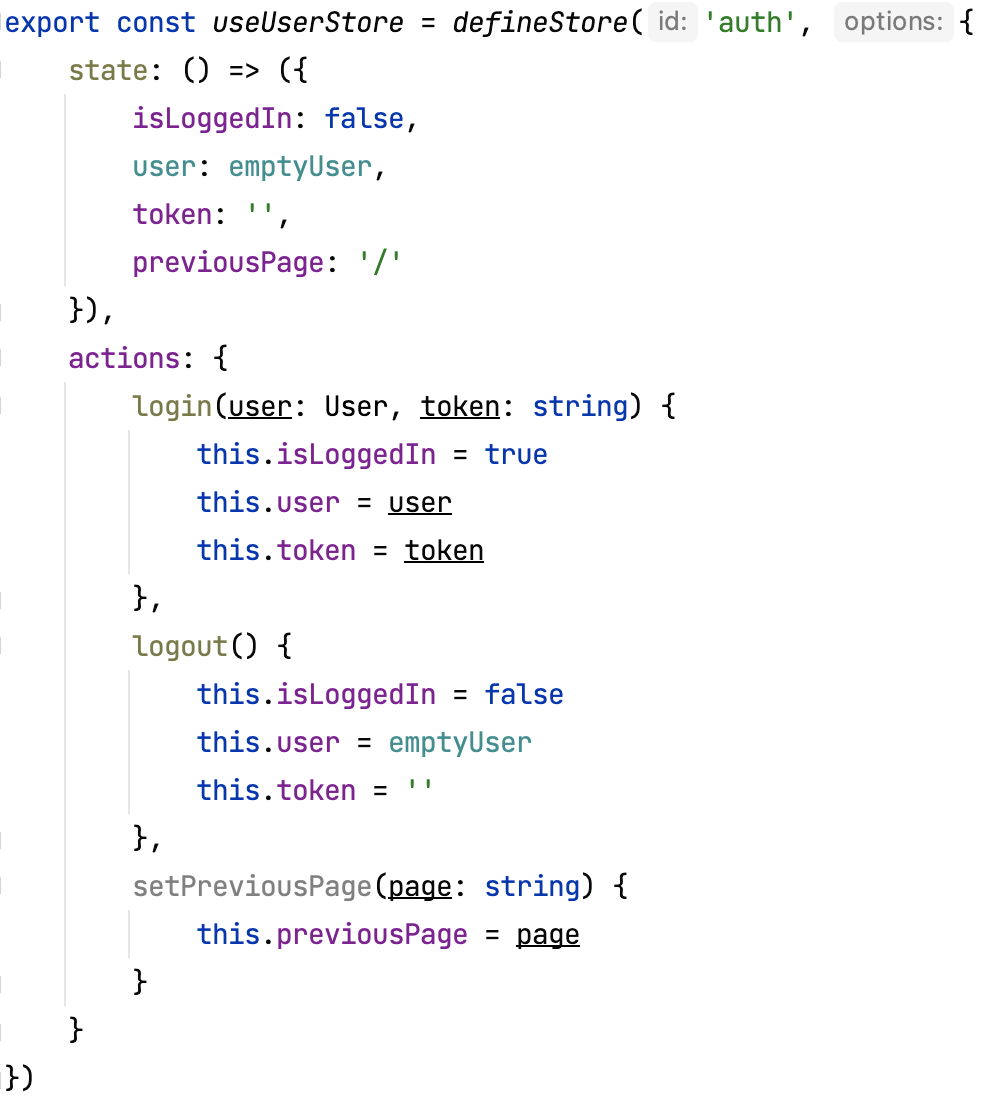
\includegraphics[scale=0.52]{../png/pinia_user.png}
\caption{Cookies setting}
\end{figure}

\noindent Pinia store is flexible and easy to use, that is an important moment because the stored information is used very often for sending requests, access control on the frontend and other.\\
Pinia storage does not provide data persistence on its own, but with a use of plugins it can enable this functionality with a use of local or session storage. Surely it is not suitable for the implementaion as I am trying to use as most secure ways to store dat as it is possible. Therefore the users data will be lost together with an access token after the page reload.\\
The BI-DBS is SPA application, meaning that page reloads are not a part of the usual functioning of the web page. However, for the case when a user does the page reload and store resets to the default values I have implemented the silent sign in. Silent sign in is shortened way of authentication and authorization process described in 4.2.5. User does not participate in this process, client just quickly gets the access token as the authorization server already knows the user and does not require to provide the credentials before the access token expires. 

\subsection{Communication with the backend and CORS}
Cross-Origin Resource Sharing(CORS) is a security mef




%%%%%%%%%%%%%%%%%%%%%%%%%%%%%%%%%%%%%%%%%%%%%%%%%%%%%%%%%%%%%%%%

\section{Role-based access control} not only visual but a security measure

\subsection{Access control for routing}

\subsection{Authentication control for requests}



%%%%%%%%%%%%%%%%%%%%%%%%%%%%%%%%%%%%%%%%%%%%%%%%%%%%%%%%%%%%%%%%




